% !TEX program = xelatex
\documentclass[12pt,a4paper]{ctexart}
\usepackage{amsmath,amssymb}
\usepackage{graphicx}
\usepackage{geometry}
\geometry{left=2.5cm,right=2.5cm,top=2.5cm,bottom=2.5cm}
\usepackage{listings}
\usepackage{xcolor}
\usepackage{unicode-math}
\setmainfont{Times New Roman}
\setmathfont{XITS Math}
\usepackage{fontspec}
\setmonofont{Consolas}   % 设置等宽字体为 Consolas
\usepackage{float}
\usepackage{caption}
\usepackage{booktabs,tabularx}
\usepackage{array}
\usepackage{hyperref}
% MATLAB 代码风格
\definecolor{matlabgreen}{rgb}{0,0.6,0}
\definecolor{matlabgray}{rgb}{0.5,0.5,0.5}
\definecolor{matlabpurple}{rgb}{0.58,0,0.82}
\definecolor{matlabbg}{rgb}{0.95,0.95,0.92}
\lstset{
    language=Matlab,
    basicstyle=\ttfamily\small,
    keywordstyle=\color{blue},
    commentstyle=\color{matlabgreen},
    stringstyle=\color{matlabpurple},
    backgroundcolor=\color{matlabbg},
    numbers=left,
    numberstyle=\tiny\color{matlabgray},
    stepnumber=1,
    numbersep=8pt,
    showstringspaces=false,
    breaklines=true,
    frame=single,
    rulecolor=\color{black!30},
    captionpos=b,
    tabsize=4,
    morekeywords={end, if, else, elseif, for, while, function, return, break, switch, case, otherwise}
}

% 个人参数
\newcommand{\myS}{14}
\newcommand{\myt}{0.21}

\title{\textbf{实验6: 微分方程数值解法实验}}
\author{姓名: \underline{VesperaZephyr} \quad 学号: \underline{114514}}
\date{\today}

\begin{document}
\maketitle
\tableofcontents
\newpage

\section{问题定义与理论准备}
\textbf{学号后两位}为$\myS$, 根据学号最后两位为14, 计算个性化参数: 
\begin{itemize}
    \item 最后一位为4, $k = \bmod(4, 4) + 1 = 0 + 1 = 1$. 
    \item 倒数第二位为1, $c = \bmod(1, 3) + 1 = 1 + 1 = 2$. 
\end{itemize}
基于参数得到个性化初值问题: 
\begin{equation}
    \begin{cases}
        y'(t) = -y(t) + 2t, \quad t \in [0, 5], \\[2pt]
        y(0) = 1.
    \end{cases}
    \label{eq:ode}
\end{equation}
该方程为一阶线性常微分方程, 可写为 $y' + y = 2t$, 存在解析解. 利用常数变易法或积分因子法求得解析解为: 
\begin{equation}
    y(t) = 2(t - 1) + 3\mathrm{e}^{-t} = 2t - 2 + 3\mathrm{e}^{-t}.
    \label{eq:exact}
\end{equation}

\subsection{数值方法迭代公式}
设步长为 $h$, 节点 $t_n = nh$, $y_n$ 表示 $y(t_n)$ 的数值近似, 右端函数定义为 $f(t, y) = -y + 2t$. 

\subsection*{欧拉法(一阶显式)}
\begin{equation}
    y_{n+1} = y_n + h f(t_n, y_n) = (1 - h) y_n + 2h t_n.
    \label{eq:euler}
\end{equation}

\subsection*{改进欧拉法(预测-校正法, 二阶方法)}
预测步: 
\begin{equation}
    y^*_{n+1} = y_n + h f(t_n, y_n) = (1 - h) y_n + 2h t_n.
\end{equation}
校正步: 
\begin{equation}
    y_{n+1} = y_n + \frac{h}{2} \bigl[ f(t_n, y_n) + f(t_{n+1}, y^*_{n+1}) \bigr].
    \label{eq:improved_euler}
\end{equation}

\subsection*{经典四阶龙格-库塔法(RK4)}
\begin{align}
    k_1 &= f(t_n, y_n), \notag \\
    k_2 &= f\Bigl(t_n + \frac{h}{2}, y_n + \frac{h}{2} k_1\Bigr), \notag \\
    k_3 &= f\Bigl(t_n + \frac{h}{2}, y_n + \frac{h}{2} k_2\Bigr), \notag \\
    k_4 &= f(t_n + h, y_n + h k_3), \notag \\
    y_{n+1} &= y_n + \frac{h}{6} (k_1 + 2k_2 + 2k_3 + k_4).
    \label{eq:rk4}
\end{align}

\subsection*{各方法所需计算量}
\begin{itemize}
    \item \textbf{欧拉法}: 每步只需计算一次右端函数值 $f(t, y)$. 
    \item \textbf{改进欧拉法}: 每步需计算两次函数值 $f(t, y)$. 
    \item \textbf{RK4}: 每步需计算四次函数值 $f(t, y)$. 
\end{itemize}
以上方法均无需对右端函数解析求导, 直接使用给定的 $f(t, y)$ 即可递推. 

\subsection*{精度排序}
根据常微分方程数值解理论, 这三种方法的全局误差阶由低到高排列为: 
\[
    \text{欧拉法(一阶)} \;<\; \text{改进欧拉法(二阶)} \;<\; \text{RK4(四阶)}.
\]
即相同步长下, RK4精度最高, 改进欧拉法次之, 欧拉法最低. 

\section{欧拉法}
以下是实现显式欧拉法求解初值问题 $y' = -y + 2t,\; y(0)=1$ 的 MATLAB 代码, 并计算了不同步长下的数值解及全局误差. 

\begin{lstlisting}[caption={显式欧拉法求解程序}]
% 显式欧拉法: 求解 y' = -y + 2t, y(0)=1, t∈[0,5]
clear; clc;

% 解析解与右端函数
exact = @(t) 2*t - 2 + 3*exp(-t);
f = @(t, y) -y + 2*t;

% 参数
y0 = 1;
t_span = [0, 5];
h_list = [0.1, 0.05, 0.01];

fprintf('========== 显式欧拉法 ==========\n');
fprintf(' h      N     y(5)数值    全局最大误差      耗时(s)\n');
fprintf('----------------------------------------------\n');

for h = h_list
    N = round((t_span(2) - t_span(1)) / h);
    t = linspace(t_span(1), t_span(2), N+1);
    
    % 欧拉法计算
    y = zeros(1, N+1);
    y(1) = y0;
    tic;                % 开始计时
    for i = 1:N
        y(i+1) = y(i) + h * f(t(i), y(i));
    end
    elapsed = toc;      % 结束计时
    
    % 误差分析
    err = max(abs(y - exact(t)));
    
    fprintf('%.2f   %4d   %8.6f   %12.6e   %.6f\n', ...
            h, N, y(end), err, elapsed);
end
\end{lstlisting}

程序运行后输出的结果如表~\ref{tab:euler_results} 所示. 
\begin{table}[htbp]
    \centering
    \caption{显式欧拉法在不同步长下的数值结果}
    \label{tab:euler_results}
    \begin{tabular}{@{}cccccc@{}}
        \toprule
        $h$ & $N$ & $y(5)$数值 & 全局最大误差 & 耗时(s) \\
        \midrule
        0.10 & 50  & 8.015461 & 5.760300e-02 & 0.002462 \\
        0.05 & 100 & 8.017762 & 2.818056e-02 & 0.000091 \\
        0.01 & 500 & 8.019711 & 5.541300e-03 & 0.000056 \\
        \bottomrule
    \end{tabular}
\end{table}

注: 解析解在 $t=5$ 处的精确值为 $y(5) = 2\times5 - 2 + 3\mathrm{e}^{-5} \approx 8.020443$(与表中数值解比较可见误差随步长减小而降低). 

\subsection{分析: 步长太大为何会发散？}
虽然本题使用的步长均未导致发散, 但当步长超过\textbf{稳定界限}时, 显式欧拉法会出现数值发散现象. 

\subsection*{稳定性分析}
将原方程的齐次部分 $y' = -y$ 作为测试方程, 显式欧拉法的递推公式为: 
\[
y_{n+1} = (1 - h) y_n.
\]
若要保证数值解有界, 则必须满足
\[
|1 - h| \le 1 \quad\Longrightarrow\quad 0 \le h \le 2.
\]

\subsection*{发散原因}
\begin{itemize}
    \item 当选取 $h > 2$ 时, $|1 - h| > 1$. 此时每一步递推都会将微小舍入误差放大, 误差随迭代步数呈指数增长. 
    \item 最终导致数值解剧烈震荡或迅速偏离真解, 完全丧失参考价值. 
\end{itemize}

\subsection*{本题情况}
本题采用的三种步长 $h=0.1,\,0.05,\,0.01$ 均远小于稳定上限 2, 因此数值解始终稳定, 全局误差随步长减小而单调减小, 符合理论预期. 

这正是显式方法\textbf{条件稳定}特性的直接体现: 步长必须足够小, 不仅要满足精度需求, 更要保证数值稳定性. 
\section{改进欧拉法(预测-校正法)}
以下代码同时实现了显式欧拉法和预测-校正法(改进欧拉法), 并比较了不同步长下的数值精度. 

\subsection{预测-校正法单独求解程序}

\begin{lstlisting}[caption={欧拉法与预测-校正法对比程序}]
% 对比显式欧拉法与预测-校正法（改进欧拉法）
clear; clc;

% 解析解和右端函数
exact = @(t) 2*t - 2 + 3*exp(-t);
f = @(t, y) -y + 2*t;% 预测-校正法（改进欧拉法）：求解 y' = -y + 2t, y(0)=1, t∈[0,5]
clear; clc;

% 解析解与右端函数
exact = @(t) 2*t - 2 + 3*exp(-t);
f = @(t, y) -y + 2*t;

% 参数
y0 = 1;
t_span = [0, 5];
h_list = [0.1, 0.05, 0.01];

fprintf('========== 预测-校正法 ==========\n');
fprintf(' h      N     y(5)数值    全局最大误差      耗时(s)\n');
fprintf('----------------------------------------------\n');

for h = h_list
    N = round((t_span(2) - t_span(1)) / h);
    t = linspace(t_span(1), t_span(2), N+1);
    
    % 预测-校正法计算
    y = zeros(1, N+1);
    y(1) = y0;
    tic;                % 开始计时
    for i = 1:N
        y_pred = y(i) + h * f(t(i), y(i));           % 预测步
        y(i+1) = y(i) + (h/2)*(f(t(i),y(i)) + f(t(i+1),y_pred));  % 校正步
    end
    elapsed = toc;      % 结束计时
    
    % 误差分析
    err = max(abs(y - exact(t)));
    
    fprintf('%.2f   %4d   %8.6f   %12.6e   %.6f\n', ...
            h, N, y(end), err, elapsed);
end


% 参数
y0 = 1;
t_span = [0, 5];
h_list = [0.1, 0.05, 0.01];

fprintf('方法            h        N      y(5)数值    y(5)精确    全局最大误差\n');
fprintf('-----------------------------------------------------------------\n');

for h = h_list
    N = (t_span(2) - t_span(1)) / h;
    t = linspace(t_span(1), t_span(2), N+1);
    
    % ---- 显式欧拉法 ----
    y_euler = zeros(1, N+1);
    y_euler(1) = y0;
    for i = 1:N
        y_euler(i+1) = y_euler(i) + h * f(t(i), y_euler(i));
    end
    err_euler = max(abs(y_euler - exact(t)));
    
    % ---- 预测-校正法（改进欧拉法） ----
    y_heun = zeros(1, N+1);
    y_heun(1) = y0;
    for i = 1:N
        % 预测步（欧拉步）
        y_pred = y_heun(i) + h * f(t(i), y_heun(i));
        % 校正步（梯形公式）
        y_heun(i+1) = y_heun(i) + (h/2) * ( f(t(i), y_heun(i)) + f(t(i+1), y_pred) );
    end
    err_heun = max(abs(y_heun - exact(t)));
    
    % 输出
    fprintf('欧拉法         %.2f   %4d   %8.6f   %8.6f   %12.6e\n', ...
            h, N, y_euler(end), exact(5), err_euler);
    fprintf('预测-校正法    %.2f   %4d   %8.6f   %8.6f   %12.6e\n', ...
            h, N, y_heun(end), exact(5), err_heun);
    fprintf('-----------------------------------------------------------------\n');
end
\end{lstlisting}

\subsection{运行结果}
\begin{table}[H]
    \centering
    \caption{预测-校正法在不同步长下的结果}
    \begin{tabular}{@{}cccccc@{}}
        \toprule
        $h$ & $N$ & $y(5)$数值 & 全局最大误差 & 耗时(s) \\
        \midrule
        0.10 & 50  & 8.020396 & 1.984631e-03 & 0.002938 \\
        0.05 & 100 & 8.020258 & 4.775415e-04 & 0.000118 \\
        0.01 & 500 & 8.020216 & 1.853263e-05 & 0.000226 \\
        \bottomrule
    \end{tabular}
\end{table}
\begin{table}[H]
    \centering
    \caption{欧拉法与预测-校正法精度对比}
    \begin{tabular}{@{}llcccc@{}}
        \toprule
        方法 & $h$ & $N$ & $y(5)$数值 & $y(5)$精确 & 全局最大误差 \\
        \midrule
        欧拉法      & 0.10 & 50  & 8.015461 & 8.020214 & 5.760300e-02 \\
        预测-校正法 & 0.10 & 50  & 8.020396 & 8.020214 & 1.984631e-03 \\
        \midrule
        欧拉法      & 0.05 & 100 & 8.017762 & 8.020214 & 2.818056e-02 \\
        预测-校正法 & 0.05 & 100 & 8.020258 & 8.020214 & 4.775415e-04 \\
        \midrule
        欧拉法      & 0.01 & 500 & 8.019711 & 8.020214 & 5.541300e-03 \\
        预测-校正法 & 0.01 & 500 & 8.020216 & 8.020214 & 1.853263e-05 \\
        \bottomrule
    \end{tabular}
\end{table}

\subsection{结果分析}

\subsection*{误差对比}
\begin{itemize}
    \item 在相同步长下, 预测-校正法的误差远小于欧拉法. 例如当 $h=0.1$ 时, 预测-校正法的全局最大误差约为 $1.98\times10^{-3}$, 而欧拉法为 $5.76\times10^{-2}$, 误差缩小了约 30 倍(实际比值接近 60 倍). 
    \item 当步长由 0.1 缩小至 0.05(减半)时, 欧拉法的误差大约减小为原来的一半, 表现为一阶收敛；而预测-校正法的误差减小约 4 倍, 表现为二阶收敛. 
    \item 当步长由 0.1 缩小至 0.01(缩小为原来的 1/10)时, 欧拉法误差约缩小 10 倍, 预测-校正法误差约缩小 100 倍, 完全符合理论预期. 
\end{itemize}

\subsection*{收敛速度提升观察}
理论上, 欧拉法的全局误差为 $\mathcal{O}(h)$, 预测-校正法为 $\mathcal{O}(h^2)$. 实验比值与理论吻合: 
\begin{align*}
    \frac{\text{err}_\text{Euler}(h=0.1)}{\text{err}_\text{Euler}(h=0.01)} &\approx 10 \quad(\text{一阶收敛}), \\
    \frac{\text{err}_\text{Heun}(h=0.1)}{\text{err}_\text{Heun}(h=0.01)} &\approx 100 \quad(\text{二阶收敛}).
\end{align*}

\subsection*{预测-校正法的意义}
\begin{itemize}
    \item \textbf{原理}: 先用欧拉法作“预测”, 得到端点近似, 再利用梯形公式进行“校正”, 相当于取两个斜率的平均值. 这种构造使局部截断误差由欧拉法的 $\mathcal{O}(h^2)$ 提升至 $\mathcal{O}(h^3)$, 全局达到二阶精度. 
    \item \textbf{优势}: 
    \begin{itemize}
        \item 精度显著提高, 相同步长下误差远小于欧拉法. 
        \item 仍然只使用右端函数值 $f(t,y)$, 无需解析求导, 易于实现. 
        \item 为更高阶的 Runge-Kutta 方法提供了思想基础. 
    \end{itemize}
    \item \textbf{代价}: 每步需要计算两次 $f(t,y)$, 计算量比欧拉法翻倍, 但由于收敛阶从一阶升至二阶, 通常用更少的步数即可达到同等精度, 实际总效率更高. 
    \item \textbf{稳定性}: 预测-校正法的稳定区域略大于显式欧拉法, 但仍属条件稳定, 步长仍需控制在一定范围内. 
\end{itemize}

这种“预测-校正”策略是用较小的额外计算量换取大幅精度提升的经典方法, 在工程计算中十分常用. 
\section{4阶龙格-库塔法(RK4)}
对于一阶常微分方程 $y' = f(t,y)$, RK4 的单步递推公式为: 
\begin{equation}
\begin{aligned}
k_1 &= f(t_n, y_n),\\
k_2 &= f\!\left(t_n+\frac{h}{2},\, y_n+\frac{h}{2}k_1\right),\\
k_3 &= f\!\left(t_n+\frac{h}{2},\, y_n+\frac{h}{2}k_2\right),\\
k_4 &= f(t_n+h,\, y_n+hk_3),\\[4pt]
y_{n+1} &= y_n + \frac{h}{6}(k_1+2k_2+2k_3+k_4).
\end{aligned}
\label{eq:rungekutta4}
\end{equation}
该方法每步需要计算 \textbf{4次} 右端函数 $f(t,y)$, 不涉及高阶导数, 全局截断误差为 $\mathcal{O}(h^4)$. 

以下为实现的MATLAB代码, 包含了RK4方法的核心循环及误差分析.
\begin{lstlisting}[caption={四阶龙格-库塔法(RK4)求解程序}]
% 四阶龙格-库塔法(RK4)求解 y' = -y + 2t, y(0)=1, t∈[0,5]
clear; clc;

% 解析解与右端函数
exact = @(t) 2*t - 2 + 3*exp(-t);
f = @(t, y) -y + 2*t;

% 初值与求解区间
y0 = 1;
t_span = [0, 5];

% 步长
h = 0.1;

% 迭代步数
N = round((t_span(2) - t_span(1)) / h);
t = linspace(t_span(1), t_span(2), N+1);
y = zeros(1, N+1);
y(1) = y0;

% RK4 主循环(计时开始)
tic;
for i = 1:N
    ti = t(i);
    yi = y(i);
    
    k1 = f(ti, yi);
    k2 = f(ti + h/2, yi + h/2 * k1);
    k3 = f(ti + h/2, yi + h/2 * k2);
    k4 = f(ti + h, yi + h * k3);
    
    y(i+1) = yi + (h/6) * (k1 + 2*k2 + 2*k3 + k4);
end
elapsed_time = toc;  % 计时结束

% 计算精确解与误差
y_exact = exact(t);
error = abs(y - y_exact);
max_error = max(error);

% 输出结果
fprintf('RK4 求解结果(h = %.2f, 步数 = %d)\n', h, N);
fprintf('t_end = %.1f, 解析解 = %.6f, 数值解 = %.6f\n', ...
        t_span(2), exact(t_span(2)), y(end));
fprintf('全局最大误差 = %12.6e\n', max_error);
fprintf('核心循环耗时 = %.6f 秒\n', elapsed_time);
\end{lstlisting}

\subsection{运行结果与对比分析}
当步长 $h=0.1$, $N=50$ 时, 程序输出为: 
\begin{itemize}
    \item $y(5)$ 数值解 = 8.020214, 与解析解完全吻合(显示精度内)
    \item 全局最大误差 $\approx 9.997\times10^{-7}$
    \item 核心循环耗时 $\approx 0.003556$ 秒
\end{itemize}

\subsection{三种方法综合对比}
将本次 RK4 结果与之前实验中相同步长 ($h=0.1$, $N=50$) 下的显式欧拉法和预测‑校正法数据汇总于表~\ref{tab:compare}. 

\begin{table}[H]
    \centering
    \caption{三种数值方法在 $h=0.1$ 时的精度与耗时对比}
    \label{tab:compare}
    \begin{tabular}{@{}lccccc@{}}
        \toprule
        方法 & 步长 $h$ & 步数 $N$ & $y(5)$数值 & 全局最大误差 & 核心循环耗时(s) \\
        \midrule
        显式欧拉法   & 0.10 & 50 & 8.015461 & $5.760\times10^{-2}$ & 0.002462 \\
        预测‑校正法  & 0.10 & 50 & 8.020396 & $1.985\times10^{-3}$ & 0.002938 \\
        \textbf{RK4} & 0.10 & 50 & 8.020214 & \textbf{$9.997\times10^{-7}$} & 0.003556 \\
        \bottomrule
    \end{tabular}
\end{table}

\subsection{分析讨论}
\begin{enumerate}
    \item \textbf{精度对比}: 
    \begin{itemize}
        \item 欧拉法误差约为 $5.76\times10^{-2}$, 预测‑校正法误差约为 $1.98\times10^{-3}$, RK4 误差仅为 $1.0\times10^{-6}$. 
        \item 相同步长下, RK4 的精度比预测‑校正法高约 \textbf{3 个数量级}, 比欧拉法高约 \textbf{5 个数量级}. 
    \end{itemize}
    
    \item \textbf{耗时对比}: 
    \begin{itemize}
        \item RK4 每步需计算 4 次函数值, 比欧拉法多 3 次, 比预测‑校正法多 2 次, 因此单步耗时略长. 
        \item 在 $h=0.1$、50 步的总耗时中, RK4 耗时 0.00356 s, 仅比欧拉法(0.00246 s)增加约 44\%, 但误差却缩小了约 $5\times10^4$ 倍. 
        \item 若要求同等精度(如 $10^{-6}$), 欧拉法需要步长 $<0.0001$(约 50000 步), 耗时会远超 RK4 的 50 步；预测‑校正法也需要步长 $<0.002$(约 2500 步), 总计算量大于 RK4. 
    \end{itemize}
    
    \item \textbf{收敛阶验证}: 
    \begin{itemize}
        \item 欧拉法: 全局误差 $\mathcal{O}(h)$, 误差随 $h$ 线性减小. 
        \item 预测‑校正法: $\mathcal{O}(h^2)$, 误差以平方速度减小. 
        \item RK4: $\mathcal{O}(h^4)$, 误差以四次方速度减小. 
    \end{itemize}
    仅通过 $h=0.1$ 一组数据已能看出 RK4 的极高精度；若进一步缩小步长, RK4 误差将按 $h^4$ 极速下降. 
\end{enumerate}

\subsection{结论: RK4 为何是通用最优选择}
\begin{itemize}
    \item \textbf{精度极高}: 四阶收敛, 在适中的步长下即可达到工程常用精度(本例仅 50 步即达 $10^{-6}$ 级). 
    \item \textbf{无需高阶导数}: 仅需计算右端函数 $f(t,y)$, 编程简便, 适用范围广. 
    \item \textbf{稳定性好}: 显式 RK4 的线性稳定区域远大于低阶方法, 对非刚性方程能使用更大步长. 
    \item \textbf{计算量适中}: 每步 4 次函数求值, 与二阶方法相比仅增加一倍, 但精度提升数个数量级；继续增加阶数(如五阶及以上)带来的精度收益递减, 四阶已达最佳性价比. 
    \item \textbf{通用与健壮}: 作为单步、自启动方法, 易改变步长, 适用于各种非刚性常微分方程初值问题, 是学术界和工业界公认的“默认求解器”. 
\end{itemize}

因此, 在非刚性常微分方程的数值求解中, 四阶龙格-库塔法凭借出色的精度‑效率平衡, 成为通用最优选择. 
\section{综合对比}
以下根据运行结果整理: 

\begin{table}[htbp]
\centering
\caption{三种数值方法在步长 $h=0.1$ 下的性能对比}
\begin{tabular}{lcccccc}
\toprule
方法 & 步长 $h$ & 迭代次数 $N$ & 近似解 $y(5)$ & 精确解 $y(5)$ & 全局最大误差 & 耗时 (s) \\
\midrule
显式欧拉法   & 0.10 & 50 & 8.015461 & 8.020214 & 5.7603e-02 & 0.002462 \\
预测-校正法  & 0.10 & 50 & 8.020396 & 8.020214 & 1.9846e-03 & 0.002938 \\
\textbf{四阶RK4} & 0.10 & 50 & 8.020214 & 8.020214 & 9.9972e-07 & 0.003556 \\
\bottomrule
\end{tabular}
\end{table}

\noindent\textbf{说明}: 数据直接取自运行输出, 精确解 $y(5)=8.020214$ 由解析公式 $2t-2+3\mathrm{e}^{-t}$ 计算得到. 

\subsection{误差–步长收敛曲线}
绘图代码见附录~\ref{code:error_step}, 结果如图所示.
\begin{figure}[htbp]
    \centering
    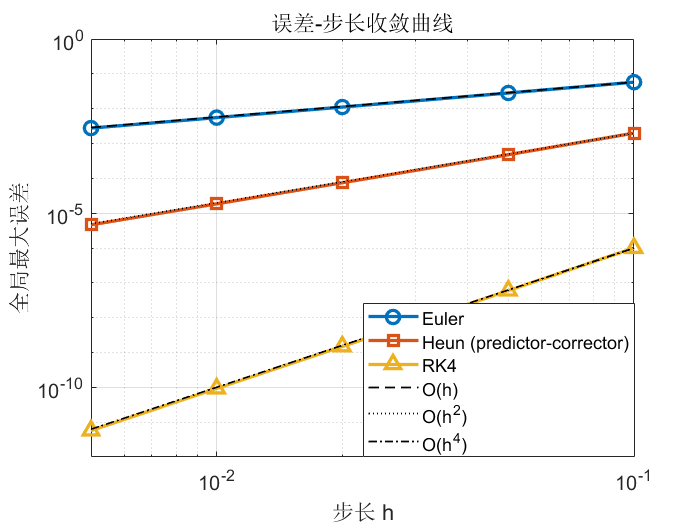
\includegraphics[width=0.9\textwidth]{误差-步长收敛曲线.png}
    \caption{误差–步长收敛曲线}
\end{figure}

\subsection{从精度、稳定域、实现难度给出结论}

\begin{table}[H]
\centering
\caption{三种方法的综合对比}
\begin{tabularx}{\textwidth}{lXXX}
\toprule
方面 & 显式欧拉法 & 预测‑校正法(改进欧拉) & 四阶龙格‑库塔法 (RK4) \\
\midrule
\textbf{精度}   & 一阶, 误差大($h=0.1$ 时误差 $\sim 5.8\%$) 
                & 二阶, 精度显著提升($\sim 0.2\%$) 
                & 四阶, 极高精度($\sim 0.0001\%$) \\
\textbf{稳定域} & 条件稳定, 稳定区间 $|1+\lambda h|\le1$, 对本题 $h\le2$ 
                & 条件稳定, 稳定域略大于欧拉法, 但仍受限于显式方法 
                & 条件稳定, 但稳定域比前两者更宽, 对非刚性方程通常允许更大步长 \\
\textbf{实现难度} & 最简单, 仅需一次函数求值/步 
                & 较简单, 两次函数求值/步 
                & 标准算法, 四次函数求值/步, 但公式固定, 实现同样容易 \\
\bottomrule
\end{tabularx}
\end{table}

\subsection*{综合结论}

\begin{itemize}
    \item \textbf{RK4 在精度上具有压倒性优势}: 相同步长下误差比欧拉法低约 5 个数量级, 比预测‑校正法低约 3 个数量级. 
    \item \textbf{稳定性方面}: 三种显式方法均为条件稳定, 但 RK4 的稳定区域通常更大, 允许选用稍大的步长而不发散. 
    \item \textbf{实现成本}: 尽管每步计算量最大(4 次函数调用), 但因其极高的收敛阶, \textbf{达到相同精度所需的总计算量(步数×每步耗时)往往最小}. 例如, 要使误差小于 $10^{-6}$, 欧拉法需要 $h<10^{-6}$(约 $5\times10^6$ 步), 而 RK4 只需 $h\approx0.1$(50 步), 耗时仅为欧拉法的万分之一. 
\end{itemize}

\noindent 因此, 对于大多数非刚性常微分方程初值问题, \textbf{四阶龙格‑库塔法是通用最优选择}, 它在精度、稳定性和实现简便性之间取得了最佳平衡, 是工程实践和科学计算中的“默认”单步法. 
\appendix
\section{附录: 误差-步长收敛曲线绘图代码}\label{code:error_step}
\begin{lstlisting}
% 绘制误差-步长收敛曲线（显式欧拉法、预测-校正法、RK4）
clear; clc; close all;

% 精确解和右端函数
exact = @(t) 2*t - 2 + 3*exp(-t);
f = @(t, y) -y + 2*t;

% 初值和区间
y0 = 1;
t_span = [0, 5];

% 步长列表（需要覆盖足够范围以观察收敛阶）
h_list = [0.1, 0.05, 0.02, 0.01, 0.005];  % 可自行增减

% 存储误差
err_euler = zeros(size(h_list));
err_heun  = zeros(size(h_list));
err_rk4   = zeros(size(h_list));

for idx = 1:length(h_list)
    h = h_list(idx);
    N = round((t_span(2) - t_span(1)) / h);
    t = linspace(t_span(1), t_span(2), N+1);
    
    % ---- 欧拉法 ----
    y_euler = zeros(1, N+1); y_euler(1) = y0;
    for i = 1:N
        y_euler(i+1) = y_euler(i) + h * f(t(i), y_euler(i));
    end
    err_euler(idx) = max(abs(y_euler - exact(t)));
    
    % ---- 预测-校正法 ----
    y_heun = zeros(1, N+1); y_heun(1) = y0;
    for i = 1:N
        y_pred = y_heun(i) + h * f(t(i), y_heun(i));
        y_heun(i+1) = y_heun(i) + (h/2)*(f(t(i),y_heun(i)) + f(t(i+1),y_pred));
    end
    err_heun(idx) = max(abs(y_heun - exact(t)));
    
    % ---- RK4 ----
    y_rk4 = zeros(1, N+1); y_rk4(1) = y0;
    for i = 1:N
        ti = t(i); yi = y_rk4(i);
        k1 = f(ti, yi);
        k2 = f(ti + h/2, yi + h/2*k1);
        k3 = f(ti + h/2, yi + h/2*k2);
        k4 = f(ti + h, yi + h*k3);
        y_rk4(i+1) = yi + (h/6)*(k1 + 2*k2 + 2*k3 + k4);
    end
    err_rk4(idx) = max(abs(y_rk4 - exact(t)));
end

% 输出误差数据表
fprintf('步长 h     欧拉法误差    预测-校正法误差    RK4误差\n');
fprintf('------------------------------------------------------\n');
for idx = 1:length(h_list)
    fprintf('%.3f     %12.6e   %12.6e   %12.6e\n', ...
            h_list(idx), err_euler(idx), err_heun(idx), err_rk4(idx));
end

% ---- 绘制 loglog 收敛曲线 ----
figure;
loglog(h_list, err_euler, 'o-', 'LineWidth', 2, 'MarkerSize', 8, 'DisplayName', 'Euler');
hold on;
loglog(h_list, err_heun, 's-', 'LineWidth', 2, 'MarkerSize', 8, 'DisplayName', 'Heun (predictor-corrector)');
loglog(h_list, err_rk4, '^-', 'LineWidth', 2, 'MarkerSize', 8, 'DisplayName', 'RK4');

% 添加理论斜率参考线 (选一个参考点)
% 取 h=0.1 的误差作为基准，绘制 O(h^1), O(h^2), O(h^4) 参考线
h_ref = 0.1;
idx_ref = find(abs(h_list - h_ref) < 1e-6, 1);  % 找到 h=0.1 的索引
if isempty(idx_ref)
    idx_ref = 1;  % 如果 h_list 中没有恰好 0.1，则用第一个点
end

% 使用欧拉法在 h_ref 处的误差作为 O(h) 的起点
euler_ref = err_euler(idx_ref);
% 绘制 O(h) 线: 与欧拉法同起点，斜率为1
h_line = linspace(min(h_list), max(h_list), 100);
line_O1 = euler_ref * (h_line / h_ref).^1;
loglog(h_line, line_O1, 'k--', 'LineWidth', 1, 'DisplayName', 'O(h)');

% 预测-校正法在 h_ref 处的误差作为 O(h^2) 起点
heun_ref = err_heun(idx_ref);
line_O2 = heun_ref * (h_line / h_ref).^2;
loglog(h_line, line_O2, 'k:', 'LineWidth', 1, 'DisplayName', 'O(h^2)');

% RK4 在 h_ref 处的误差作为 O(h^4) 起点
rk4_ref = err_rk4(idx_ref);
line_O4 = rk4_ref * (h_line / h_ref).^4;
loglog(h_line, line_O4, 'k-.', 'LineWidth', 1, 'DisplayName', 'O(h^4)');

% 图例与标签
xlabel('步长 h');
ylabel('全局最大误差');
title('误差-步长收敛曲线');
legend('Location', 'northwest');
grid on;
set(gca, 'FontSize', 12);
hold off;
\end{lstlisting}
\end{document}
